\documentclass[12pt, twoside]{article}
\usepackage[letterpaper, margin=1in, headsep=0.5in]{geometry}
\usepackage[english]{babel}
\usepackage[utf8]{inputenc}
\usepackage{amsmath}
\usepackage{amsfonts}
\usepackage{amssymb}
\usepackage{tikz}
%\usetikzlibrary{quotes, angles}

\usepackage{graphicx}
\usepackage{enumitem}
\usepackage{multicol}

\usepackage{fancyhdr}
\pagestyle{fancy}
\fancyhf{}
\renewcommand{\headrulewidth}{0pt} % disable the underline of the header

\fancyhead[RE]{\thepage}
\fancyhead[RO]{\thepage \\ Name: \hspace{3cm}}
\fancyhead[LO]{BECA / Dr. Huson / 10th Grade Geometry\\* Unit 5: Transformation, dilation, and scale \\* 8 November 2019}

\begin{document}
\subsubsection*{5.4 Do Now: Similar triangles, dilation ratios}
 \begin{enumerate}

  \item On the graph below, dilate the triangle $ABC$ by a factor of $\frac{3}{2}$ centered on the origin.\\
    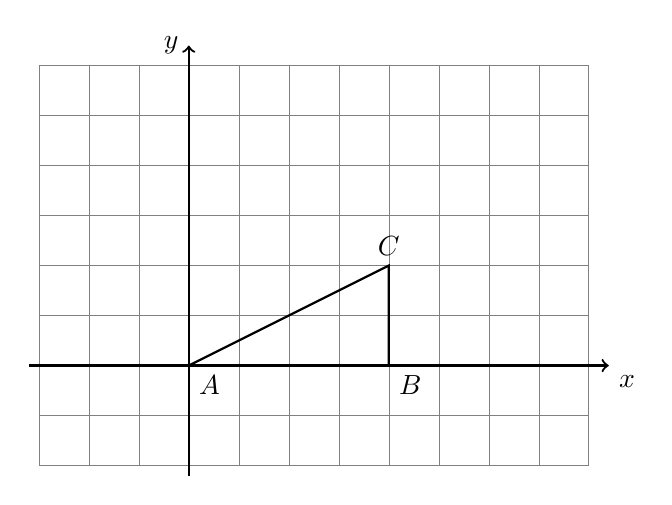
\begin{tikzpicture}[scale=.635]
      \draw [help lines] (-3,-2) grid (8,6);
      \draw [thick, ->] (-3.2,0) -- (8.4,0) node [below right] {$x$};
      \draw [thick, ->] (0,-2.2)--(0,6.4) node [left] {$y$};
      \draw [thick] (0,0)node[below right]{$A$}--
       (4,0)node[below right]{$B$}--
         (4,2)node[above]{$C$}--cycle;
    \end{tikzpicture}
   \vspace{2cm}


 \item Triangle $ABC$ is dilated with a factor of $\frac{5}{3}$ centered at $A$, yielding $\triangle ADE$, as shown. Given $AB=9$, $BC=12$, and $AC=15$. \\[0.25cm] Find $AD$, $AE$, and $DE$. \vspace{0.5cm}
 \begin{flushright}
     \begin{tikzpicture}[scale=0.7]
       \draw [thick]
       (0,0)node[left]{$B$}--
       (8,0)node[above right]{$C$}--
       (2,6)node[left]{$A$}--cycle;
       \draw [thick]
       (0,0)--
       (-1,-3)node[left]{$D$}--
       (11,-3)node[above right]{$E$}--(8,0);
       \node at (4,0)[below]{$12$};
       \node at (5.3, 3)[right]{$15$};
       \node at (0.3, 2.8)[above]{$9$};
     \end{tikzpicture}
   \end{flushright}

\newpage

\item The coordinates of the endpoints of $\overline{AB}$ are $A(1,2)$ and $B(4,2)$. Determine the length of $\overline{A'B'}$, the image of  $\overline{AB}$, after a dilation of $k=2$ centered at the origin.\\[0.25cm]
Draw and label the two line segments,  $\overline{AB}$ and  $\overline{A'B'}$, on the set of axes below.
  \vspace{1cm}
  \begin{center}
    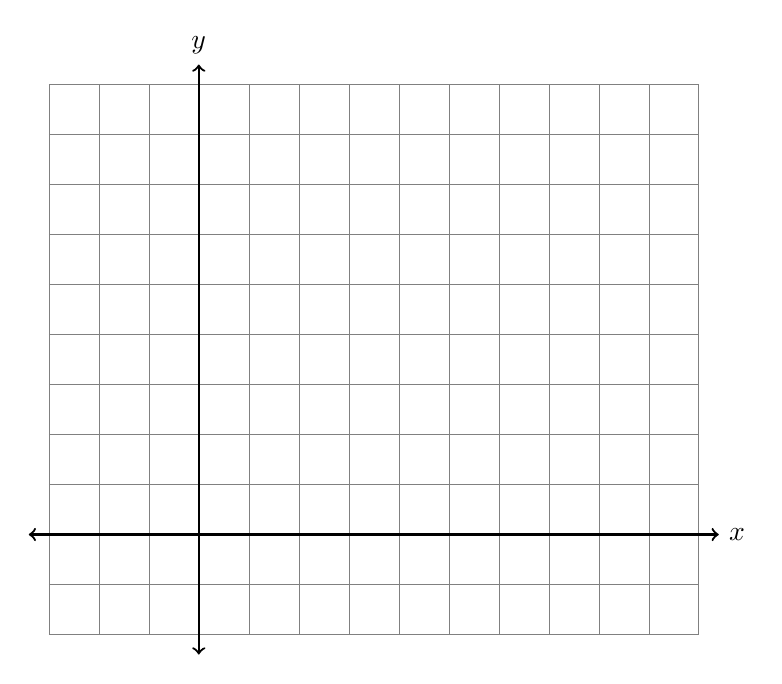
\begin{tikzpicture}[scale=.635]
      \draw [help lines] (-3,-2) grid (10,9);
      \draw [thick, <->] (-3.4,0) -- (10.4,0) node [right] {$x$};
      \draw [thick, <->] (0,-2.4)--(0,9.4) node [above] {$y$};
    \end{tikzpicture}
  \end{center}


\item Triangle $ADE$ is drawn with $\overline{BC} \parallel \overline{DE}$, as shown. Given $AB=5$, $BC=7$, $AC=8$, and $BD=5$. \\[0.25cm] Find $CE$, $AE$, and $DE$. \vspace{1cm}
\begin{flushright}
   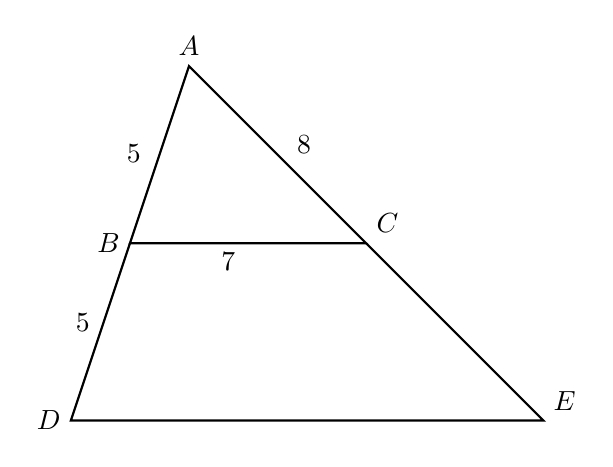
\begin{tikzpicture}[scale=0.5]
     \draw [thick]
     (0.5,1.5)node[left]{$B$}--
     (6.5,1.5)node[above right]{$C$}--
     (2,6)node[above]{$A$}--cycle;
     \draw [thick]
     (0.5,1.5)--
     (-1,-3)node[left]{$D$}--
     (11,-3)node[above right]{$E$}--(6.5,1.5);
     \node at (3,1.5)[below]{$7$};
     \node at (4.5, 4)[right]{$8$};
     \node at (0.6, 3.3)[above]{$5$};
     \node at (-0.7, -1)[above]{$5$};
   \end{tikzpicture}
 \end{flushright}

\newpage
 \item Given $\triangle ABC \sim \triangle DEF$. $m\angle A = 40^\circ$ and $m\angle E = 35^\circ$.\\
 Find the measure of $\angle C$. \vspace{3cm}

 \item Given $\triangle ABP$ and $\triangle JKP$ as shown below. $\overline{AB} \parallel \overline{JK}$. $AP=5.7$, $JP=11.4$, and $JK=14.8$. Find $AB$.
 \begin{flushright}
   \begin{tikzpicture}[scale=1.4]
       \draw [thick]
         (0.25,-1)node[right]{$B$}--
         (-0.5,2)node[left]{$K$}--
         (4,0)node[right]{$J$}--
         (0,0)node[above right]{$P$}--
         (-2,0)node[left]{$A$}--cycle;
     \end{tikzpicture}
     \end{flushright}
     \vspace{3cm}

   \begin{multicols}{2}
    [\item A translation maps triangle $CAT$ onto triangle $DOG$.] \vspace{0.5cm}
      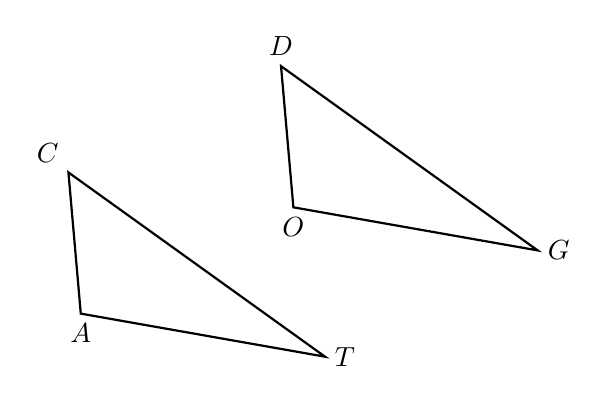
\begin{tikzpicture}[scale=0.9]
        \coordinate [label=above left:$C$](A) at (95:2);
        \coordinate [label=below:$A$](B) at (0, 0);
        \coordinate [label=right:$T$](C) at (-10:3.5);
        \draw [thick] (A)--(B)--(C)--cycle;
  
        \draw [thick, xshift=3cm, yshift=1.5cm] (95:2) node[above]{$D$}--
        (0,0) node[below]{$O$}--
        (-10:3.5) node[right]{$G$}--cycle;
      \end{tikzpicture}\\
      Fill in the blank with the corresponding object.
      \begin{enumerate}
        \item $A \rightarrow$ \rule{2cm}{0.15mm}
        \item $\angle CTA \cong$ \rule{2cm}{0.15mm}
        \item \rule{2cm}{0.15mm} $\cong \overline {DG}$
        \item Justify $\triangle CAT \cong \triangle DOG$.
      \end{enumerate}
    \end{multicols}  \vspace{4cm}

\newpage

\item Using a compass and straightedge, construct the perpendicular bisector of $\overline{BB'}$  \\[0.25cm]
What transformation has been applied to map $\triangle ABC$ on to $\triangle A'B'C'$? \vspace{2cm}
    \begin{center}
    \begin{tikzpicture}[scale=.8]
      %\draw [thick, <->] (-7.4,0) -- (10.4,0) node [right] {$x$};
      %\draw [thick, <->] (0,-6.4)--(0,10.4) node [above] {$y$};

      \draw [thick]
      (5,-1) node[below left] {$A$}--
      (8,2) node[right] {$B$}--
      (1,0) node[below left] {$C$}--cycle;

      \draw [thick]
      (-1,5) node[right] {$A'$}--
      (2,8) node[above] {$B'$}--
      (0,1) node[below left] {$C'$}--cycle;

    \end{tikzpicture}
  \end{center}

\item Triangle $ABC$ is dilated with a factor of $\frac{3}{2}$ centered at $A$, yielding $\triangle ADE$, as shown. Given $AB=10$, $BC=12$, and $AC=14$. \\[0.25cm] Find $AD$, $AE$, and $DE$. \vspace{1cm}
\begin{flushright}
    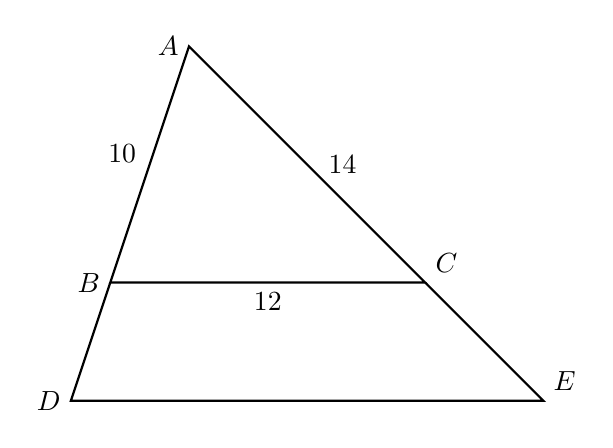
\begin{tikzpicture}[scale=0.5]
      \draw [thick]
      (0,0)node[left]{$B$}--
      (8,0)node[above right]{$C$}--
      (2,6)node[left]{$A$}--cycle;
      \draw [thick]
      (0,0)--
      (-1,-3)node[left]{$D$}--
      (11,-3)node[above right]{$E$}--(8,0);
      \node at (4,0)[below]{$12$};
      \node at (5.3, 3)[right]{$14$};
      \node at (0.3, 2.8)[above]{$10$};
    \end{tikzpicture}
  \end{flushright}

\end{enumerate}
\end{document}
